\documentclass[11pt,a4paper]{article}
\usepackage[margin=22mm]{geometry}
\usepackage{amsmath,amssymb,booktabs,array}
\usepackage[T1]{fontenc}
\usepackage{lmodern}
\usepackage{tikz}
\usetikzlibrary{arrows.meta,positioning}
\usepackage{hyperref}
\usepackage{xurl}
\hypersetup{colorlinks=true,linkcolor=blue,urlcolor=blue}
\setlength{\parindent}{0pt}
\setlength{\parskip}{5pt}
\newcommand{\VDD}{V_{\mathrm{dd}}}
\newcommand{\VTH}{V_t}
\newcommand{\IL}{I_L}
\newcommand{\size}{\left(W/L\right)}
\title{Introduction to VLSI Design\\2024 Homework 2 --- Worked Solutions}
\author{Independent derivation with reference-answer review}
\date{13 October 2026}
\begin{document}
\begin{center}
{\Large\bfseries Introduction to VLSI Design\\[3pt]
2024 Homework 2 --- Worked Solutions}\\[6pt]
{\small Independent derivation with reference-answer review\quad$\cdot$\quad13 October 2026}
\end{center}
\textbf{Scope.} The supplied 2024 Homework 2 contains two analytical problems.
The answers below use its stated constant-threshold, constant-leakage and
constant-on-resistance assumptions. Supplementary HSPICE decks are supplied
separately; the CIC BSIM3 model must not be confused with those assumptions.

\section*{1. Non-ideal effect}
\subsection*{(a) Precharge voltage}
For $\mathrm{Pre}=0$, the PMOS connects BL to $\VDD$ without an NMOS-style
high-level threshold loss. For $\mathrm{SL}=1$, take the NMOS gate to be
$\VDD$. As the storage-node voltage $V_C$ rises,
\[
 V_{GS,n}=\VDD-V_C.
\]
In the question's threshold-cutoff approximation, charging stops at
$V_{GS,n}=\VTH$. Therefore
\begin{equation}
 \boxed{V_C(0)=\VDD-\VTH.}\label{eq:precharge}
\end{equation}
The threshold loss is across the access NMOS, not the precharge PMOS.
Here $\VTH$ is the threshold stipulated by the question. If body effect is
included, it becomes an implicit equation
$V_C=\VDD-V_t(V_{SB}=V_C)$ rather than a subtraction using the zero-body-bias
threshold. Subthreshold conduction also removes an ideal abrupt cutoff.

\subsection*{(b) Stored-data retention time}
Let $t=0$ be the end of precharge. Assume that the storage-side NMOS
junction removes a constant current $\IL>0$ from the capacitor, with all
other storage-node leakage and loading neglected. Charge conservation gives
\[
 Q=CV_C,\qquad C\frac{dV_C}{dt}=-\IL,
 \qquad V_C(t)=\VDD-\VTH-\frac{\IL}{C}t.
\]
The boundary at which a stored high can no longer exceed the stated
buffer threshold is $V_C(t_{\mathrm{ret}})=0.4\VDD$. Hence
\begin{equation}
 \boxed{t_{\mathrm{ret}}=\frac{C(0.6\VDD-\VTH)}{\IL},
 \quad\text{provided }\VTH<0.6\VDD.}\label{eq:retention}
\end{equation}
The data is safely high for $0\leq t<t_{\mathrm{ret}}$ in this ideal model;
equality is the switching boundary, with no noise margin. If
$\VTH\geq0.6\VDD$, the initial stored voltage does not exceed the threshold,
so there is no positive guaranteed high-retention interval. If $\IL=0$ and
the initial margin is positive, this ideal model predicts infinite retention.
No numerical $C$, $\VTH$, $\VDD$ or $\IL$ is specified by the assignment.

\textbf{Important topology qualification.} In the original Fig.~1, the
buffer input is attached to BL, while $C$ is on the other side of the
access NMOS. When SL is low, these are separate nodes:
\begin{center}
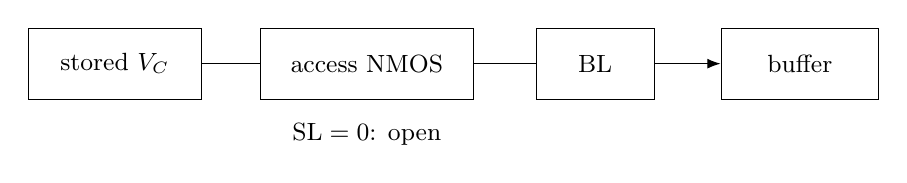
\begin{tikzpicture}[>=Latex,font=\small]
 \node[draw,minimum width=22mm,minimum height=9mm] (c) at (0,0) {stored $V_C$};
 \node[draw,minimum width=27mm,minimum height=9mm] (s) at (3.2,0) {access NMOS};
 \node[draw,minimum width=15mm,minimum height=9mm] (b) at (6.1,0) {BL};
 \node[draw,minimum width=20mm,minimum height=9mm] (buf) at (8.7,0) {buffer};
 \draw (c)--(s); \draw (s)--(b); \draw[->] (b)--(buf);
 \node at (3.2,-.9) {$\mathrm{SL}=0$: open};
\end{tikzpicture}
\end{center}
Equation~\eqref{eq:retention} is the intended \emph{stored-charge} answer,
under an implicit ideal read that exposes the storage voltage to the buffer
without appreciable disturbance. It is not a prediction of continuously
observed Out while both transistors remain off. That literal interpretation
needs BL capacitance, BL leakage and a read protocol, none of which are given.
For example, upon reselecting a cell with BL capacitance $C_{BL}$ initially
at $V_{BL,0}$, ideal charge sharing would give
\[
 V_{\mathrm{share}}=\frac{CV_C+C_{BL}V_{BL,0}}{C+C_{BL}},
\]
before considering threshold loss or buffer loading. The threshold condition
must then be imposed on the actual read voltage. No extra factor of two
is applied to $\IL$: only the storage-connected junction directly discharges
$C$ while the access transistor is off.

\textbf{Illustrative calculation, not assignment data.} Choosing
$\VDD=1.8\,\mathrm{V}$, $\VTH=0.45\,\mathrm{V}$,
$C=20\,\mathrm{fF}$ and $\IL=1\,\mathrm{pA}$ gives
\[
 V_C(0)=1.35\,\mathrm{V},\quad V_{\mathrm{switch}}=0.72\,\mathrm{V},
 \quad t_{\mathrm{ret}}=12.6\,\mathrm{ms}.
\]
The deck \texttt{q1\_constant\_leakage.sp} implements this ideal capacitor
and current-source model directly, not the full access-transistor circuit.

\section*{2. Logic gate}
\subsection*{(a) Boolean function}
The PMOS gate is tied to ground, so the pull-up remains on. The two NMOS
devices form parallel pull-down paths. Either high input pulls the output
low, while both inputs low leave the output high. Thus the intended logic is
\begin{equation}
 \boxed{Y=\overline{A+B}=\bar A\,\bar B,\quad\text{a pseudo-NMOS NOR gate}.}
\end{equation}
It is ratioed logic: correct low levels require sufficiently strong NMOS
devices, and low-output states draw static supply current.
\begin{center}
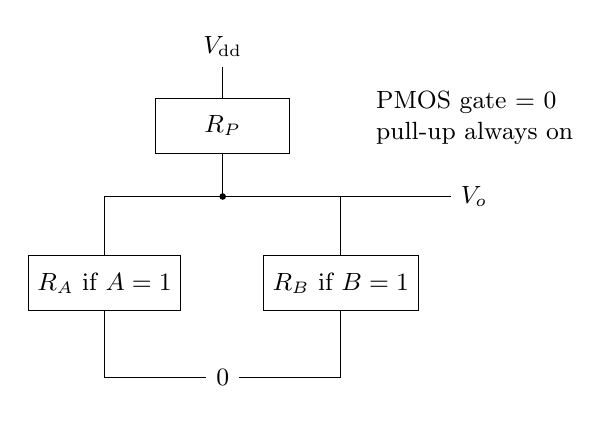
\begin{tikzpicture}[font=\small]
 \node (dd) at (0,2.8) {$\VDD$};
 \node[draw,minimum width=17mm,minimum height=7mm] (p) at (0,1.8) {$R_P$};
 \coordinate (y) at (0,.9);
 \node[draw,minimum width=17mm,minimum height=7mm] (a) at (-1.5,-.2) {$R_A$ if $A=1$};
 \node[draw,minimum width=17mm,minimum height=7mm] (b) at (1.5,-.2) {$R_B$ if $B=1$};
 \node (g) at (0,-1.4) {$0$};
 \draw (dd)--(p)--(y); \fill (y) circle(1.2pt);
 \draw (y)--(2.9,.9) node[right]{$V_o$};
 \draw (y)-|(a); \draw (y)-|(b);
 \draw (a)|-(g); \draw (b)|-(g);
 \node[align=left] at (3.2,1.9) {PMOS gate = 0\\pull-up always on};
\end{tikzpicture}
\end{center}

\subsection*{(b) Transistor sizing}
The phrase ``smallest voltage of logic 0 is $0.2\VDD$'' is interpreted as
the \emph{maximum acceptable logic-low voltage}, $V_{OL,\max}=0.2\VDD$.
A smallest allowed low voltage would not define a sensible sizing requirement,
because ground is also a valid low. This interpretation is also used in the
provided handwritten answer.

Let $S_0$ be an arbitrary reference aspect ratio, and define
\[
 s_A=\frac{(W/L)_{nA}}{S_0},\quad
 s_B=\frac{(W/L)_{nB}}{S_0},\quad
 s_p=\frac{(W/L)_p}{S_0}.
\]
For equal reference sizes the assignment specifies $R_p=2R_n$.
With resistance inversely proportional to aspect ratio,
\[
 R_A=\frac{R_n}{s_A},\qquad
 R_B=\frac{R_n}{s_B},\qquad
 R_P=\frac{2R_n}{s_p}.
\]
For $A=1,B=0$, the constant-resistance divider gives
\[
 \frac{V_{10}}{\VDD}=\frac{R_A}{R_P+R_A}
 =\frac{s_p}{s_p+2s_A}\leq0.2
 \quad\Longrightarrow\quad s_A\geq2s_p.
\]
The $A=0,B=1$ case independently requires $s_B\geq2s_p$. Therefore
\begin{equation}
 \boxed{\size_{nA}\geq2\size_p,\qquad
        \size_{nB}\geq2\size_p.}\label{eq:sizing}
\end{equation}
The minimum symmetric ratios are $(W/L)_{nA}=(W/L)_{nB}=2(W/L)_p$.
For equal channel lengths, each NMOS width is at least twice the PMOS width.
The assignment fixes ratios, not unique absolute widths or lengths.

At the boundary, write $R_A=R_B=R$ and $R_P=4R$. The complete truth table is
\begin{center}
\begin{tabular}{ccccc}
\toprule
$A$ & $B$ & Pull-down resistance & $V_o/\VDD$ & Logic \\
\midrule
0 & 0 & open & 1 & 1 \\
0 & 1 & $R$ & $1/5=0.2$ & 0 \\
1 & 0 & $R$ & $1/5=0.2$ & 0 \\
1 & 1 & $R/2$ & $1/9\simeq0.1111$ & 0 \\
\bottomrule
\end{tabular}
\end{center}
The worst low occurs with only one NMOS on; sizing from the two-on case
would be insufficient. The equality solution has no additional margin to
the stated $0.2\VDD$ limit. Larger NMOS-to-PMOS ratios reduce the low voltage
in this resistor model, at the cost of more input capacitance and area.

\textbf{Numerical resistor check.} For $\VDD=1.8\,\mathrm{V}$,
$R=1\,\mathrm{k\Omega}$, $R_P=4\,\mathrm{k\Omega}$:
\[
 (V_{00},V_{01},V_{10},V_{11})=(1.8,0.36,0.36,0.20)\,\mathrm{V}.
\]
The one-on supply current is $1.8/(4000+1000)=0.36\,\mathrm{mA}$;
the corresponding total static power is $0.648\,\mathrm{mW}$.
These absolute resistor values are illustrative and are not extracted from CIC.

\section*{Supplementary numerical validation and reproducibility}
\begin{center}
\begin{tabular}{p{.40\linewidth}p{.51\linewidth}}
\toprule
File & Purpose \\
\midrule
\texttt{q1\_constant\_leakage.sp} & Constant leakage and initial-voltage abstraction; measures threshold-crossing time. \\
\texttt{q2\_constant\_resistance.sp} & Four exact resistor-divider input cases. \\
\texttt{q2\_cic018\_tt.sp} & BSIM3 pseudo-NMOS NOR, TT, $25^\circ$C, $1.8$ V; sweeps NMOS/PMOS aspect-ratio ratios 1, 2, 3, 4, 6 and 8. \\
\texttt{reproduce.py} & Runs all decks, records exit status and raw console logs; separately writes closed-form expectations. \\
\bottomrule
\end{tabular}
\end{center}
The CIC deck uses $L_n=L_p=0.18\,\mu\mathrm{m}$, $W_p=0.5\,\mu\mathrm{m}$,
and $W_n=rW_p$. It measures all four DC-settled output voltages and supply
currents. A valid numerical low must satisfy $V_{01},V_{10},V_{11}\leq0.36$ V
at this chosen supply; a small output number alone does not verify the high state.
The voltage-source currents are negated to report positive current delivered
by each supply. Ideal voltage inputs are used and output loading is zero.

BSIM3 has voltage-dependent currents, body effects and subthreshold current;
it does not impose the problem's constant $R_p=2R_n$ rule.
Consequently, a BSIM3 voltage at ratio two need not equal $0.2\VDD$ and cannot
replace the analytical answer in Eq.~\eqref{eq:sizing}.
The local library is included in a protected section to avoid expanding it
into a public listing; the model file itself is not part of this submission.
The model is identified locally as CIC 0.18\,$\mu$m, BSIM3, version 1.3,
21 January 2008. For BSIM3 model physics, see the
\href{https://www2.eecs.berkeley.edu/Pubs/TechRpts/1998/ERL-98-51.pdf}{UC Berkeley BSIM3v3.2 manual}.

\textbf{Actual execution.} All three decks completed successfully with
PrimeSim HSPICE S-2021.09 on 13 October 2026 (exit code 0).
The measured ideal retention is $12.600025$ ms, versus the closed-form
$12.600000$ ms: relative error $1.98\times10^{-6}$, due to transient startup
and integration. At $12.6$ ms the measured voltage is $0.72000125$ V.
The ideal resistor deck measures exactly the four voltages listed above
to its reported precision.

The following are actual CIC TT measurements at $25^\circ$C:
\begin{center}
\begin{tabular}{rrrrr}
\toprule
$r=W_n/W_p$ & $V_{00}$ (V) & $V_{01}=V_{10}$ (V) & $V_{11}$ (V) & $P_{01}$ (mW) \\
\midrule
1 & 1.800000 & 0.176482 & 0.078389 & 0.242883 \\
2 & 1.800000 & 0.078122 & 0.036908 & 0.245440 \\
3 & 1.800000 & 0.049900 & 0.024040 & 0.246127 \\
4 & 1.800000 & 0.036566 & 0.017786 & 0.246445 \\
6 & 1.800000 & 0.023779 & 0.011676 & 0.246746 \\
8 & 1.800000 & 0.017604 & 0.008684 & 0.246891 \\
\bottomrule
\end{tabular}
\end{center}
For example, at ratio two the measured one-on supply current is
$0.1363557$ mA. Even ratio one passes the low-voltage criterion for this
particular TT model and bias; this neither changes the assignment's
constant-resistance requirement nor establishes a minimum ratio across
process corners, voltage and temperature.

The files \path{*_measurements.csv} are parsed from HSPICE measurement
tables, while \path{analytic_expected.csv} contains only closed-form
calculations. \path{simulation_status.csv} and
\path{validation_summary.json} record successful execution without local
license metadata. Run \texttt{python reproduce.py} to repeat the simulations;
raw simulator files go to a temporary local directory by default.
\path{validate_results.py} compares the ideal results to the equations,
checks all sampled CIC output levels and symmetry, and verifies static
power against supply current. All 43 numerical checks passed; their
observations and tolerances are in \path{validation_checks.csv}.

\section*{Reference-answer comparison}
The provided handwritten \texttt{VLSI\_HW2.pdf} was reviewed after deriving
the solution independently. Its precharge and retention formulas agree
with Eqs.~\eqref{eq:precharge}--\eqref{eq:retention}, and its NOR identification,
$R_P=4R_N$ boundary, size ratio two, and $V_{11}=\VDD/9$ agree with the
constant-resistance derivation. Those results are retained.

The final answer adds the initial-readability condition, the BL isolation
qualification, the general size inequality, and the distinction between
ideal resistors and a BSIM3 device calculation. The handwritten text near
the start of part 2(a) says the NMOS turns on for ``$A=1\land B=1$'';
for the parallel network, either individual NMOS turns on with its own
high input. The subsequent truth-case analysis in that answer correctly
uses the OR condition. No numerical HSPICE results appear in that reference,
and none have been inferred from it.
\end{document}
